%%%%%%%%%%%%%%%%%%%%%%%%%%%%%%%%%%%%%%%%%%%%%%%%%%%%%%%%%%%%%
%% HEADER
%%%%%%%%%%%%%%%%%%%%%%%%%%%%%%%%%%%%%%%%%%%%%%%%%%%%%%%%%%%%%
\documentclass[9pt]{beamer}

\usetheme{Diuf}
\usepackage{thumbpdf}
\usepackage{wasysym}
\usepackage{ucs}
\usepackage{multicol}
\usepackage{subfigure}
\usepackage{pgf,pgfarrows,pgfnodes,pgfautomata,pgfheaps,pgfshade}
\usepackage{verbatim}
\usepackage{tikz}
\usepackage{algorithmic}
\usepackage{algorithm}
\usetikzlibrary{calc}

\newtheorem{concl}{Conclusion}

\definecolor{darkgreen}{rgb}{0.,0.6,0.}
\newcommand{\textevert}{\textcolor{darkgreen}}

\begin{document}

\title[]{Sparsification of Parallel Spectral Clustering\footnote{\tiny{This
work was performed using HPC resources from CALMIP (Grant 2012-p0989)}}}
\author{Sandrine Mouysset\\
Ronan Guivarch}
\institute{APO Team\\
Institut de Recherche en Informatique de Toulouse\\
University of Toulouse}
\date{VECPAR'12 - 10th International Meeting
High Performance Computing for Computational Science}


\setbeamertemplate{footline}

\frame{ \titlepage}

%%%%%%%%%%%%%%%%%%%%%%%%%%%%%%%%%%%%%%%%%%%%%%
%%%%%%%%%%%%%%%%%%%%%%%%%%%%%%%%%%%%%%%%%%%%%%
\frame{\frametitle{Clustering}
\begin{block}{Goal:}
{\it Partition a $n \times p$ data set in K clusters to obtain larger within-cluster affinity and lower between-clusters affinity}
\end{block}
\bigskip
Some clustering methods based on: 
\medskip
\begin{itemize}
\item geometrical properties: K-means...\\
\smallskip
\item spectral properties: \alert{Spectral clustering}...
\end{itemize}

\begin{center}
\begin{tabular}{ccc}
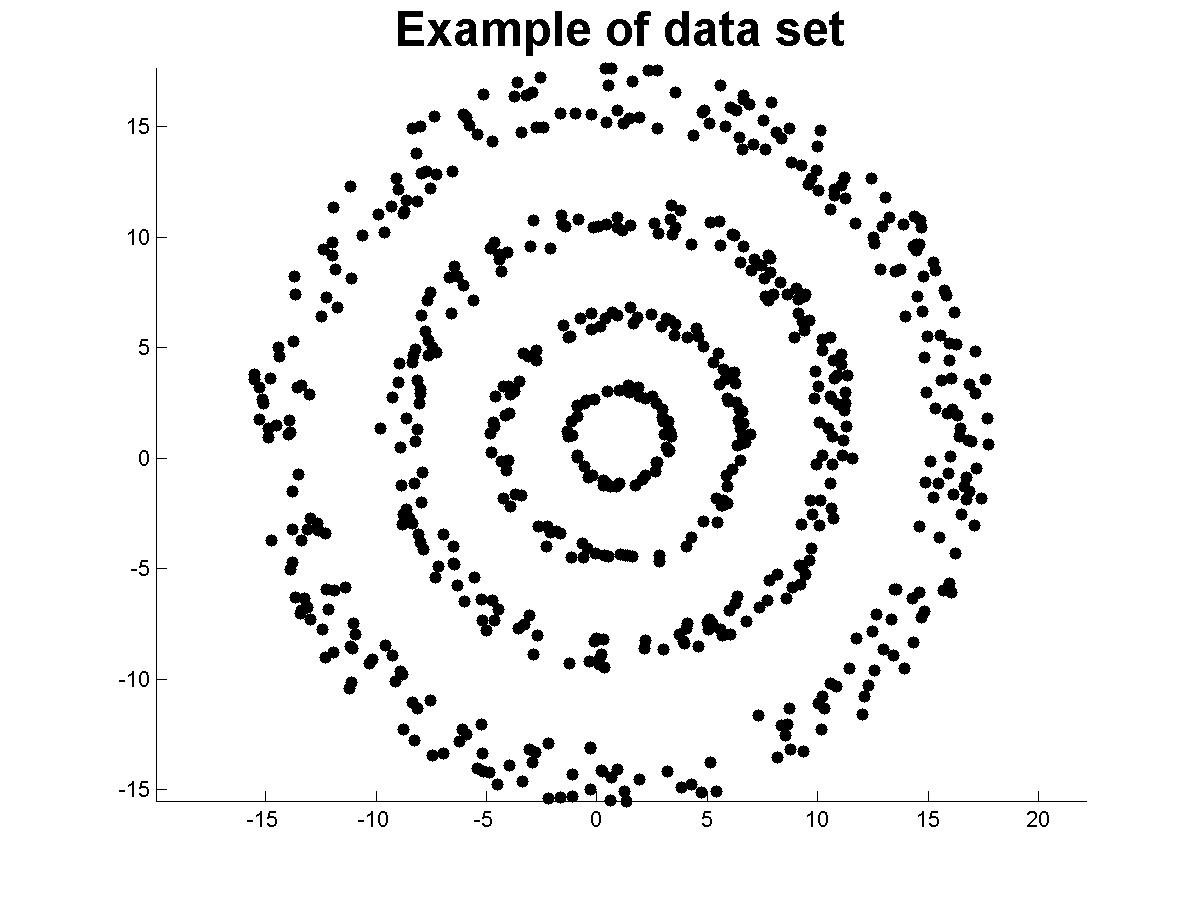
\includegraphics[width=0.32\linewidth]{cibledata} & 
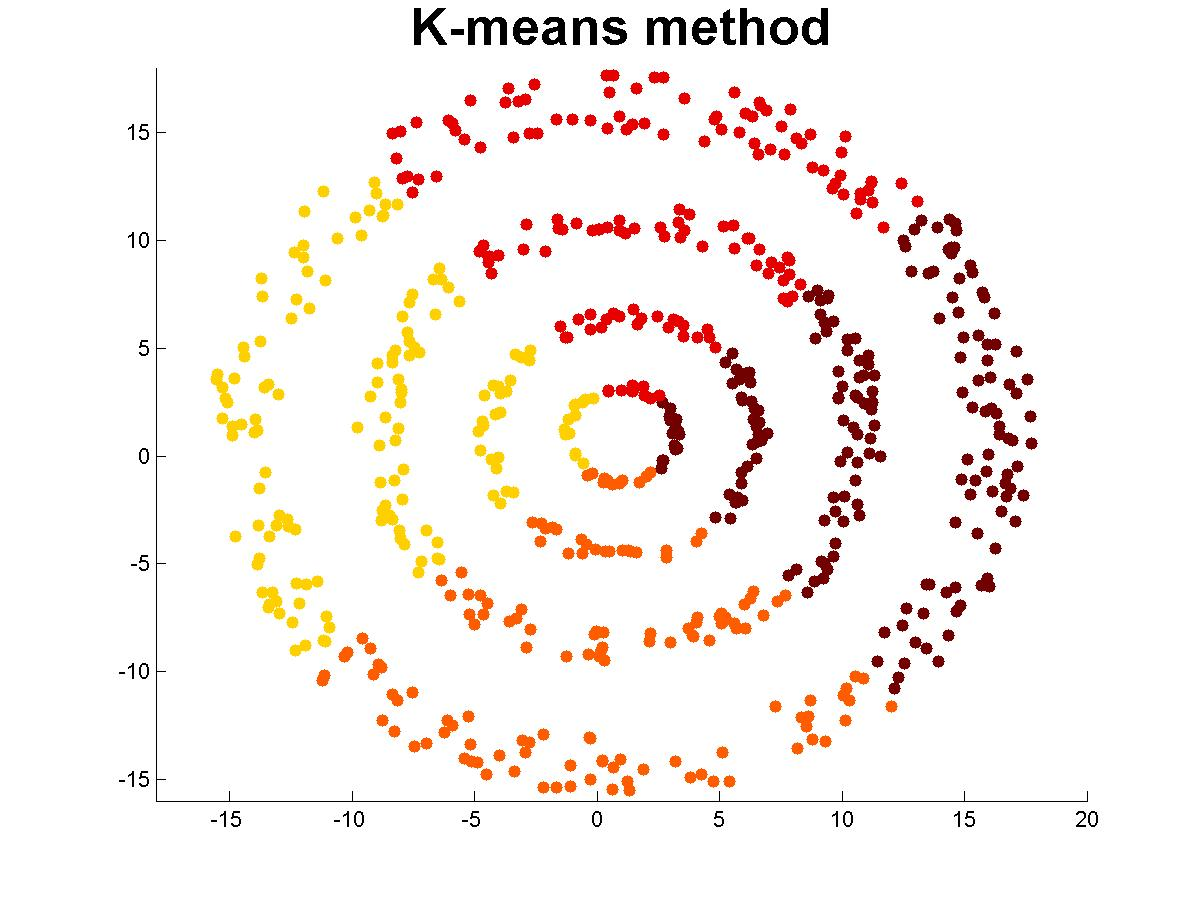
\includegraphics[width=0.32\linewidth]{casciblekmeans} &
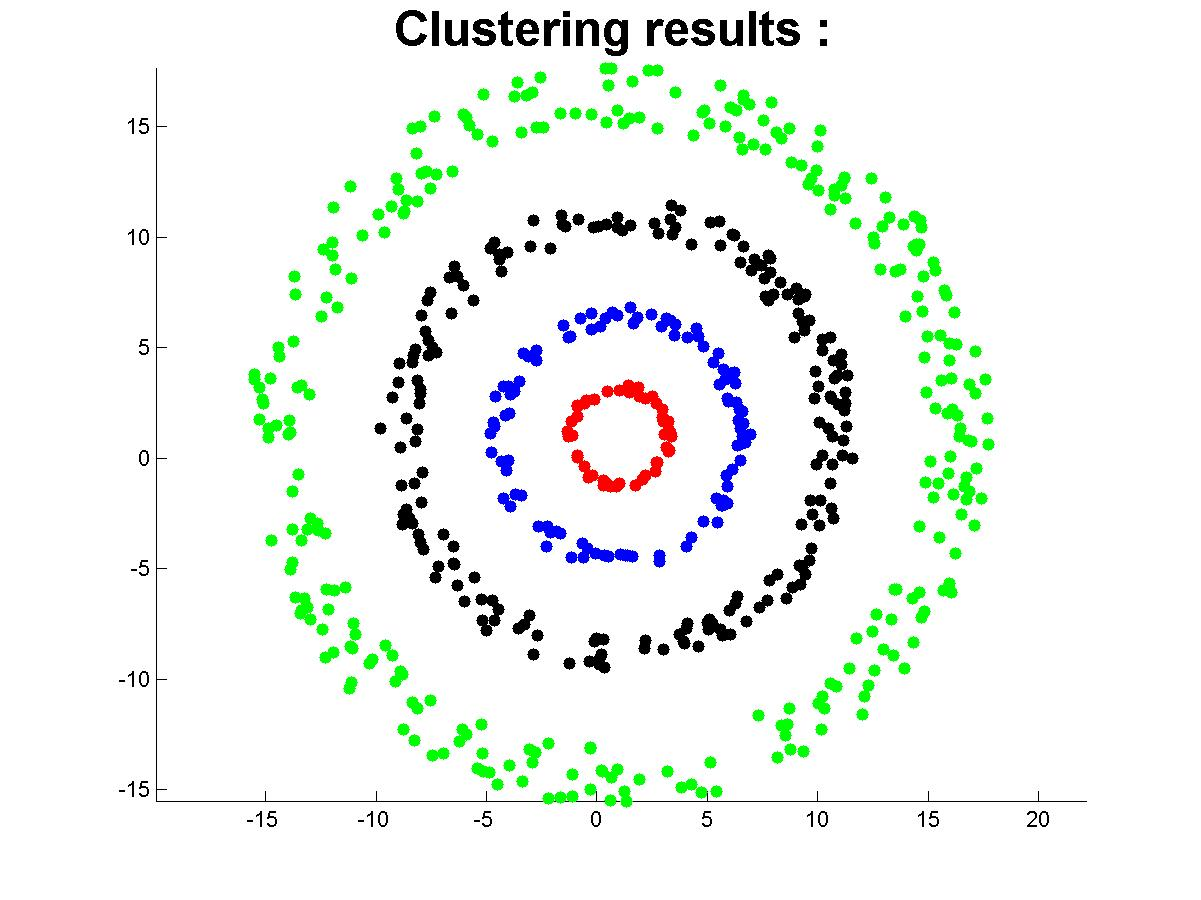
\includegraphics[width=0.32\linewidth]{cible}
\end{tabular}
\end{center} 
}

\frame{\frametitle{Outline}

\begin{itemize}
\item Spectral Clustering
\item Parallel Spectral Clustering
\item Sparsification
\item Numerical Results
\item Conclusion \& Future Works
\end{itemize}

}
%%%%%%%%%%%%%%%%%%%%%%%%%%%%%%%%%%%%%%%%
\frame{\frametitle{Spectral Clustering: introduction}
\begin{block}{Spectral Clustering}
select dominant eigenvectors of a parametrized \alert{affinity matrix $A$} in order to build a \alert{low-dimensional} data space wherein data points are \alert{grouped} into clusters
\end{block}
\bigskip
Main difficulties:
\begin{itemize}
\item How to (automatically) separate clusters one from the other?\\
\alert{$\qquad \rightarrow$ Look for some full-unsupervising process}
\medskip 
\item How to perform clustering on large datasets (image segmentation)?\\
\alert{$\qquad \rightarrow$ Parallelization using domain decomposition}
\end{itemize}
}
%%%%%%%%%%%%%%%%%%%%%%%%%
\frame{\frametitle{Algorithm {\it Ng, Jordan and Weiss}[2002]}
%\begin{exampleblock}{}
%\begin{itemize}
%\item[$\rightarrow$] {\bf Spectral Clustering: theoretical points and through a parallel implementation}
%\end{itemize}
%\end{exampleblock}
%\medskip
\begin{multicols}{2}
\begin{figure}[!h]
\begin{center}
\only<1>{\subfigure[Data set (n=300)]{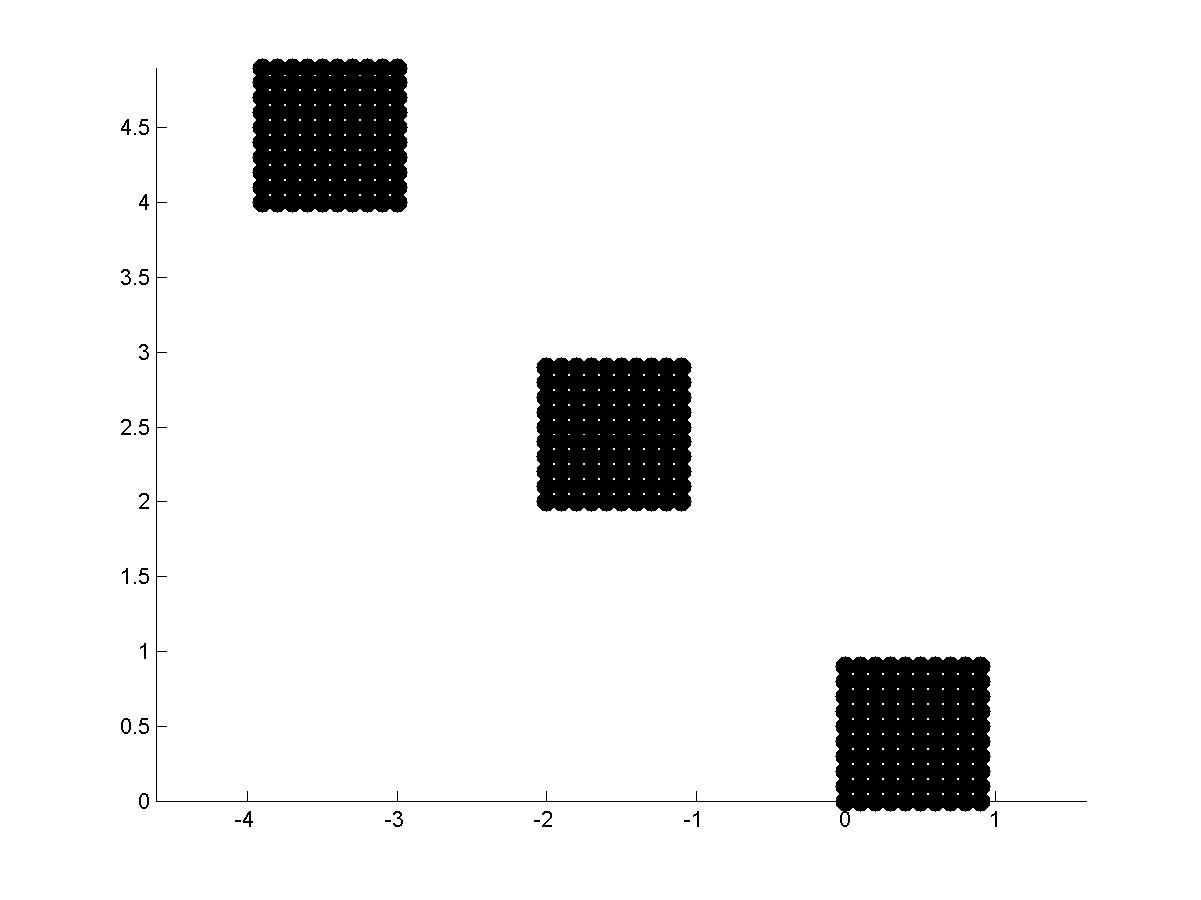
\includegraphics[width=0.95\linewidth]{3blocksblack}}}
\only<2>{\subfigure[Affinity matrix (step 2)]{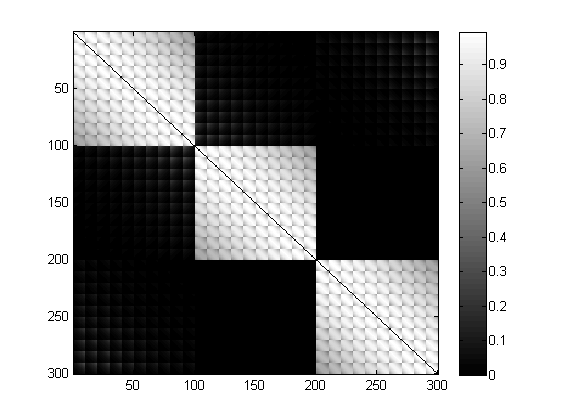
\includegraphics[width=0.95\linewidth]{affinite_3blocs_ord_g}}}
\only<3>{\subfigure[$Y$'s rows (step 4)]{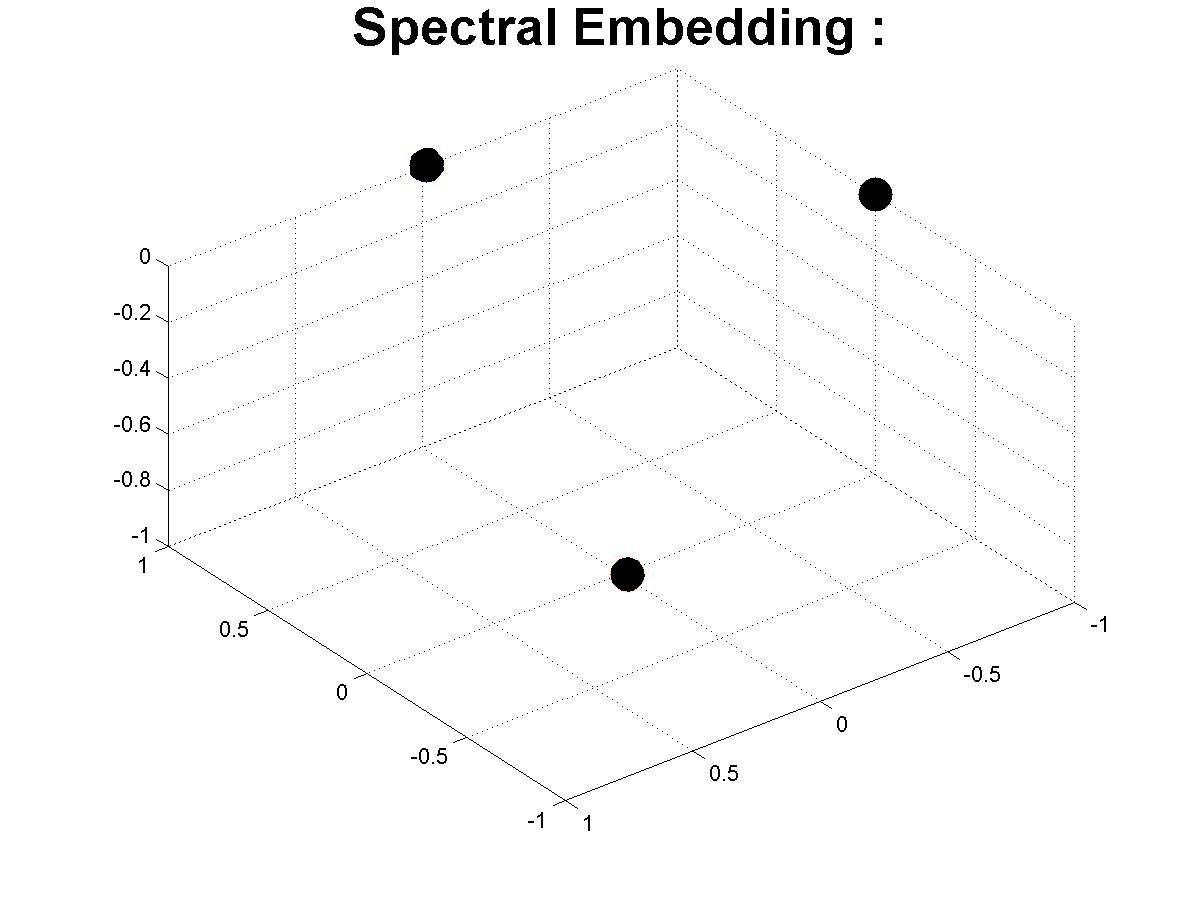
\includegraphics[width=0.95\linewidth]{3blocksembedstep1}}}
\only<4>{\subfigure[Clustering of $Y$'s rows (step 5)]{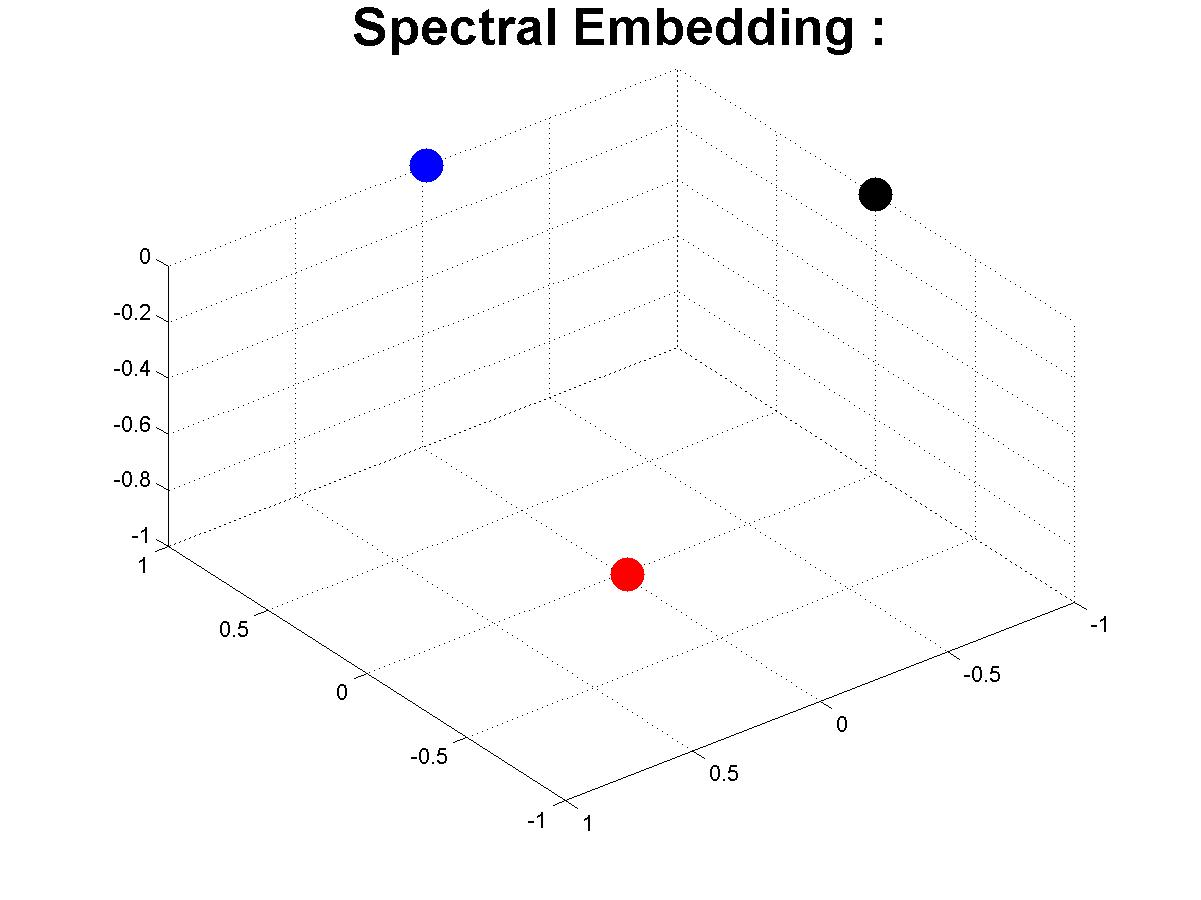
\includegraphics[width=0.95\linewidth]{3blocksembed}}}
\only<5->{\subfigure[3 well-separated clusters (step 6)]{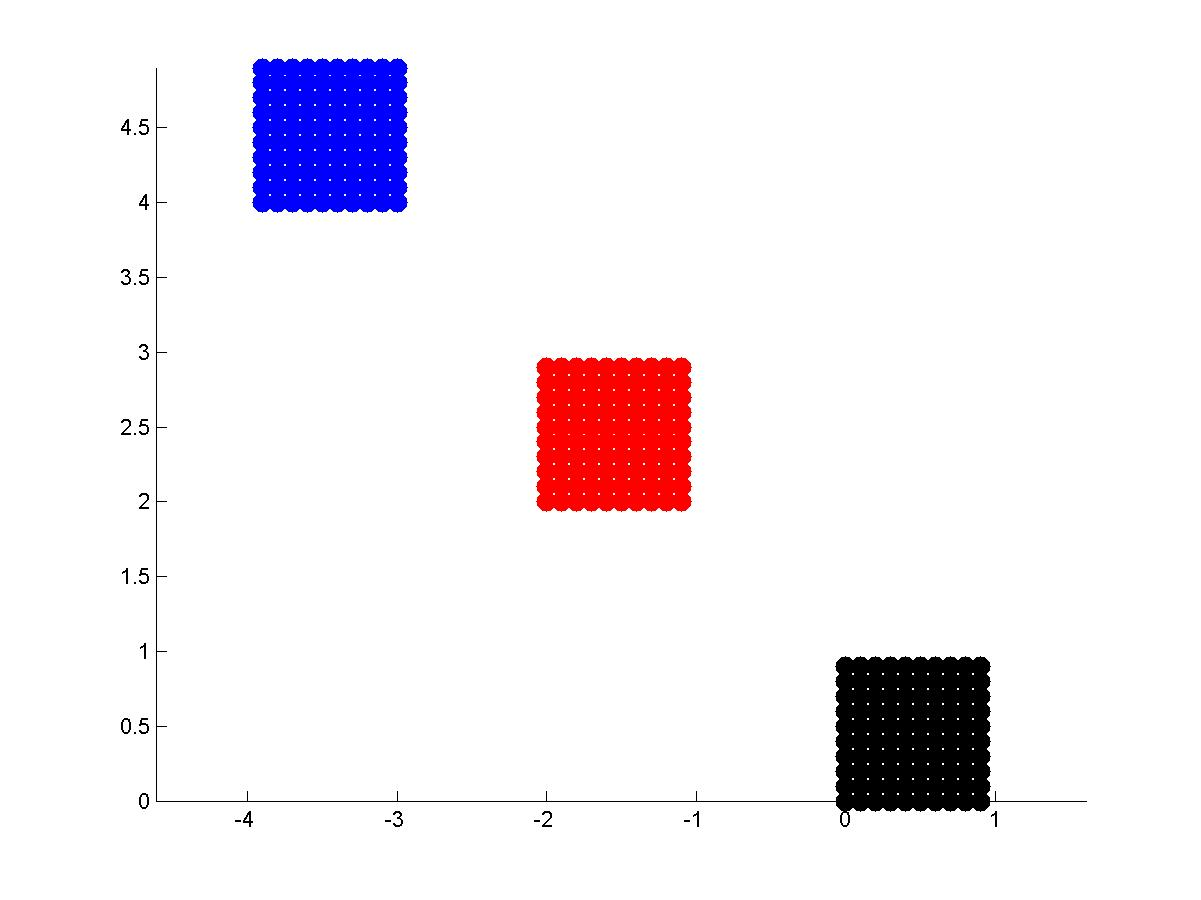
\includegraphics[width=0.95\linewidth]{3blocks}}}
\end{center} 
\end{figure}
\begin{enumerate}
\alert<1>{\item $\,$} Input: data set $\{x_i\}_{i=1..n}$
\pause
\alert<2>{\item $\,$} Form the \textevert{Gaussian affinity matrix} $\textevert{A}\in\mathbb{R}^{n\times n}$ defined by:
$$A_{ij}=\begin{cases}
\displaystyle e^{-\left\|x_i-x_j\right\|^2/2 \alert{\bf \sigma}^2} \text{\  if $i\neq j$,}\\
0 \ \text{otherwise}
\end{cases}$$
(\alert{$\sigma$ to be defined})
\alert<2>{\item $\,$}  Construct the normalized matrix: $L=D^{-1}A$ with $D_{i,i}=\sum_{j=1}^n A_{ij}\ $
\pause
\alert<3>{\item $\,$}  Construct the matrix $X=[X_1X_2..X_k]\in
\mathbb{R}^{n\times k}$ by stacking the \alert{$k$} "largest'' eigenvectors of $L$. Form the matrix Y by normalizing each of the X's rows. (\alert{$k$ to be defined})
\pause
\alert<4>{\item $\,$}  Treat each row of Y as a point in $\mathbb{R}^{k}$ and cluster them in $k$ clusters via {\it K-means} method
\pause
\alert<5>{\item $\,$}  Assign the original point $x_i$ to cluster $j$ if and only if row $i$ of the matrix Y was assigned to cluster $j$. 
\end{enumerate}
\end{multicols}
}
%%%%%%%%%%%%%%%%%%%%
\frame{\frametitle{Parameters to define}

\begin{alertblock} {Two main problems arise:}
\begin{itemize}
\item Choice of the Gaussian affinity parameter $\sigma$
\item Estimating the number of clusters $k$
\end{itemize}
\end{alertblock}

\begin{block}{Gaussian affinity parameter}
Heuristic based on the density of data distribution which includes both number of data $n$ and its dimension $p$:
$$\sigma=\frac{\max_{1\leq i,j \leq n}  \| x_i - x_j \|}{n^{\frac{1}{p}}}$$
\end{block}

\begin{block}{Number of clusters $k$}
For different values of $k$
\begin{itemize}
\item Index the affinity matrix per cluster which provides a block structure;
\item Compute the mean ratio between all off-diagonal blocks and the diagonal ones in Frobenius norms;
\item Reach the optimal value $k$ which minimizes the mean ratio.
\end{itemize}
\end{block}
\bigskip
$\qquad \rightarrow$ full-unsupervising process
}

%%%%%%%%%%%%%%%%%%%%%%%%%
\frame{\frametitle{Interpretation of Gaussian affinity matrix as discretization of Heat kernel}

\begin{itemize}
  \item Affinity between two data points $x_i$ and $x_j$ 
$$A_{ij}=\exp\left(\frac{-\left\|x_i-x_j\right\|^2}{2 \sigma^2}\right)$$
  \item Heat kernel in \alert{free space}
 $$K_t(x-y)=(4\pi t)^{-\frac{p}{2}}\exp\left(-\frac{\|x-y\|^2}{4t}\right)$$

  \item Finite Element Theory
\end{itemize}
}

\frame{\frametitle{Interpretation of Gaussian affinity matrix as discretization of Heat kernel}
\vspace{-0.2cm}
\begin{center}
Eigenfunctions for Heat equation with \alert{Dirichlet boundary conditions}:\\
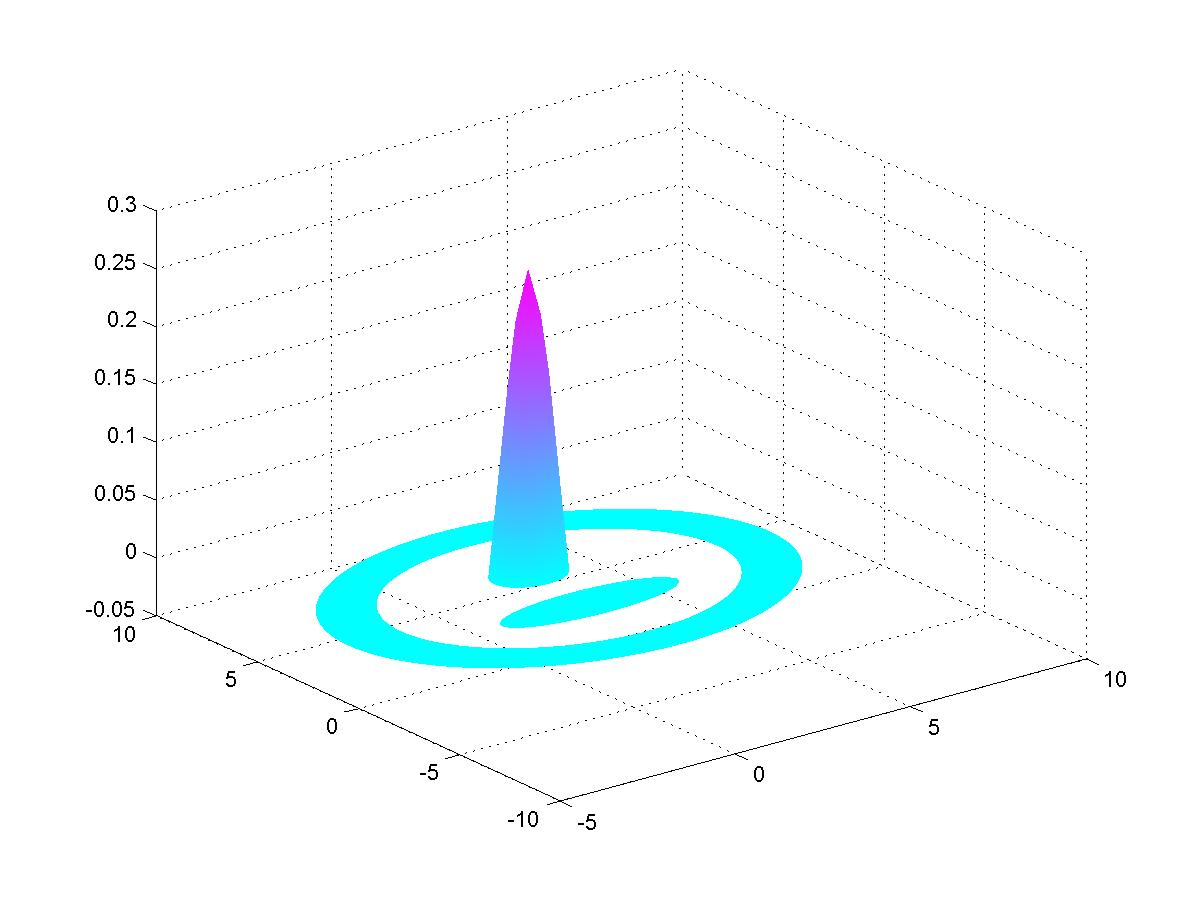
\includegraphics[width=0.28\linewidth]{eigpdedonut4} 
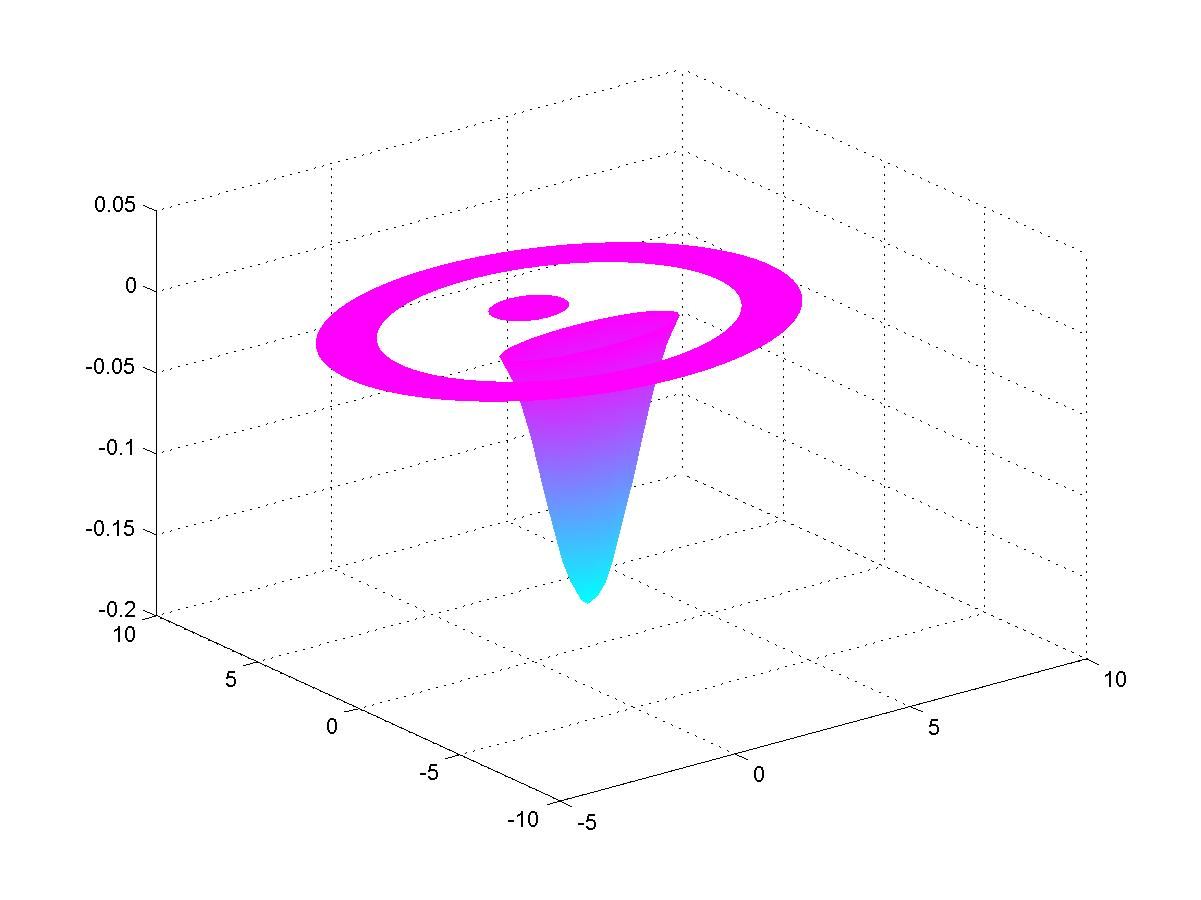
\includegraphics[width=0.28\linewidth]{eigpde2donut4} 
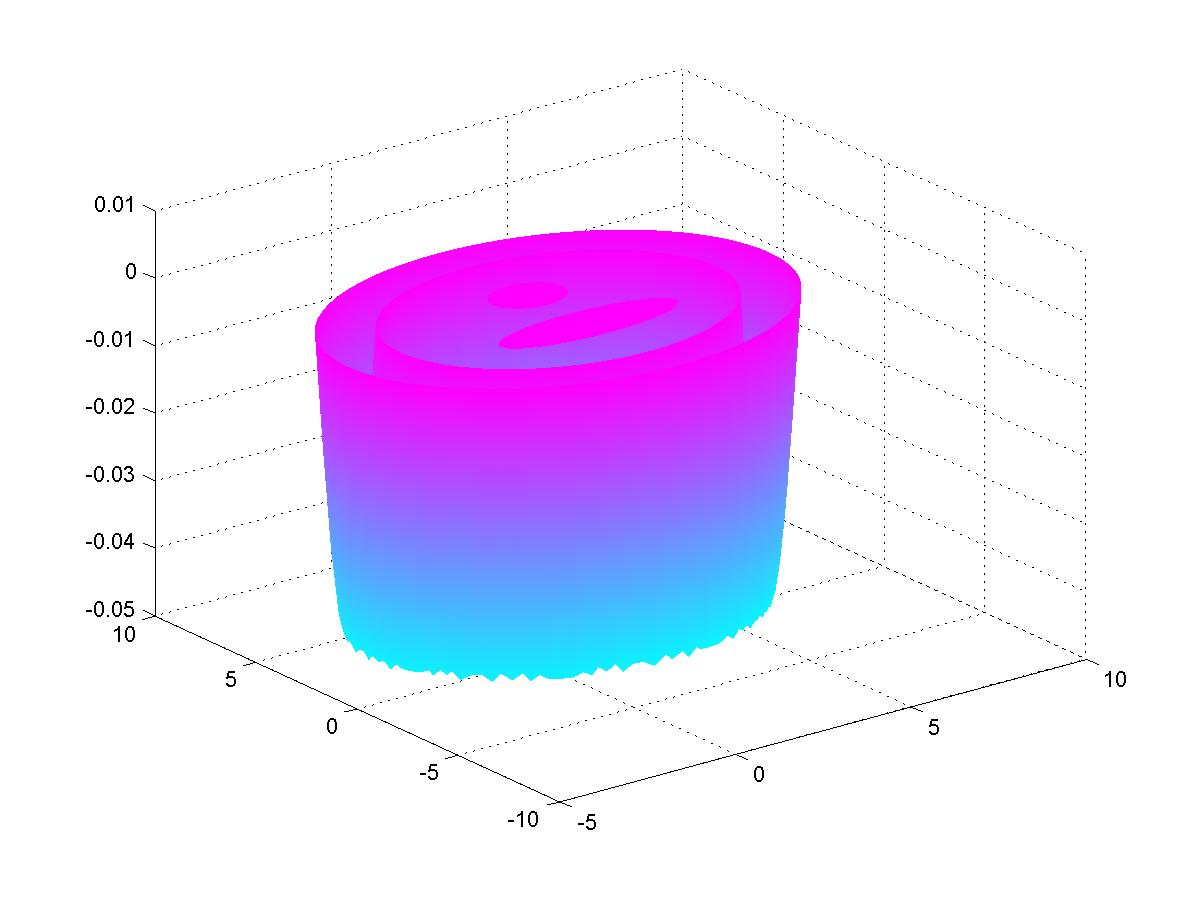
\includegraphics[width=0.28\linewidth]{eigpde3donut4} \\
Eigenvectors of the affinity matrix $A$: \\
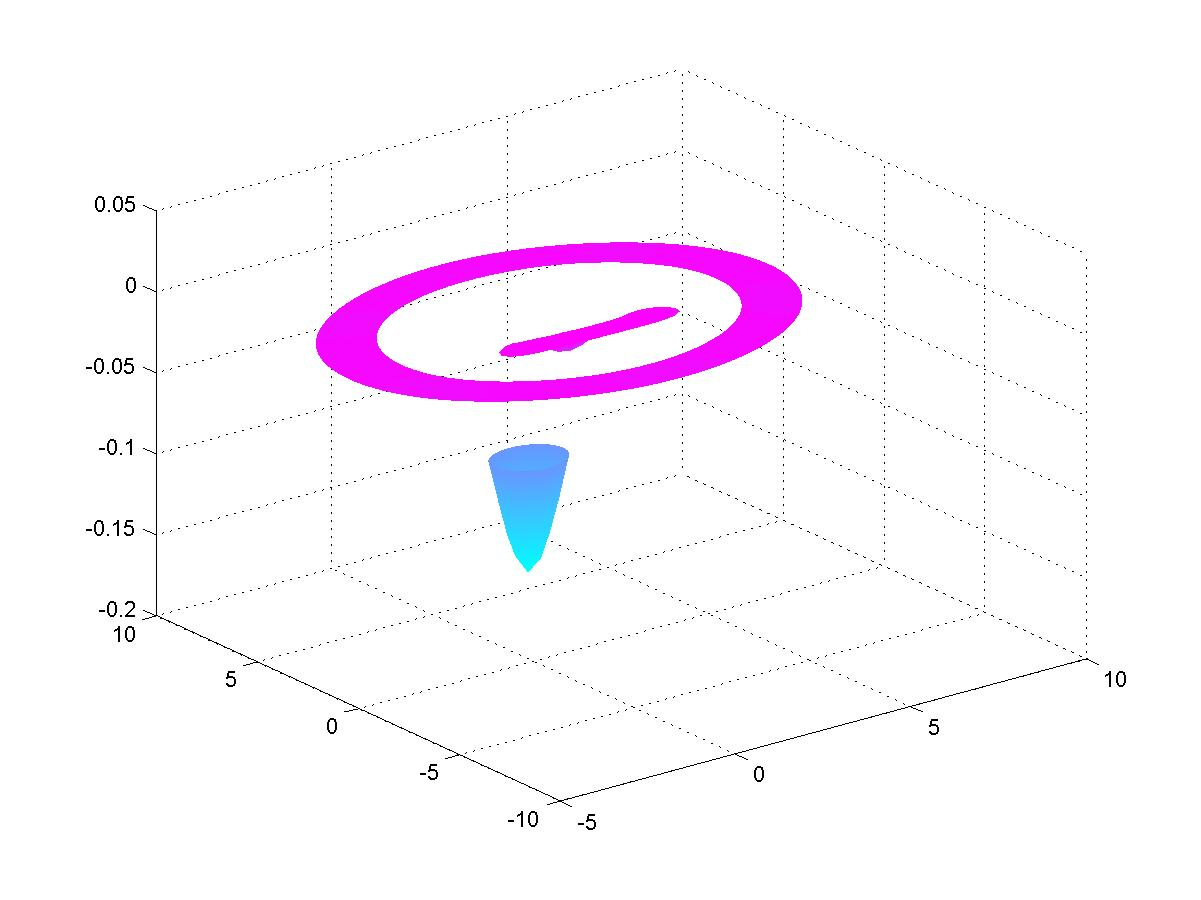
\includegraphics[width=0.28\linewidth]{eigspec3donut4} 
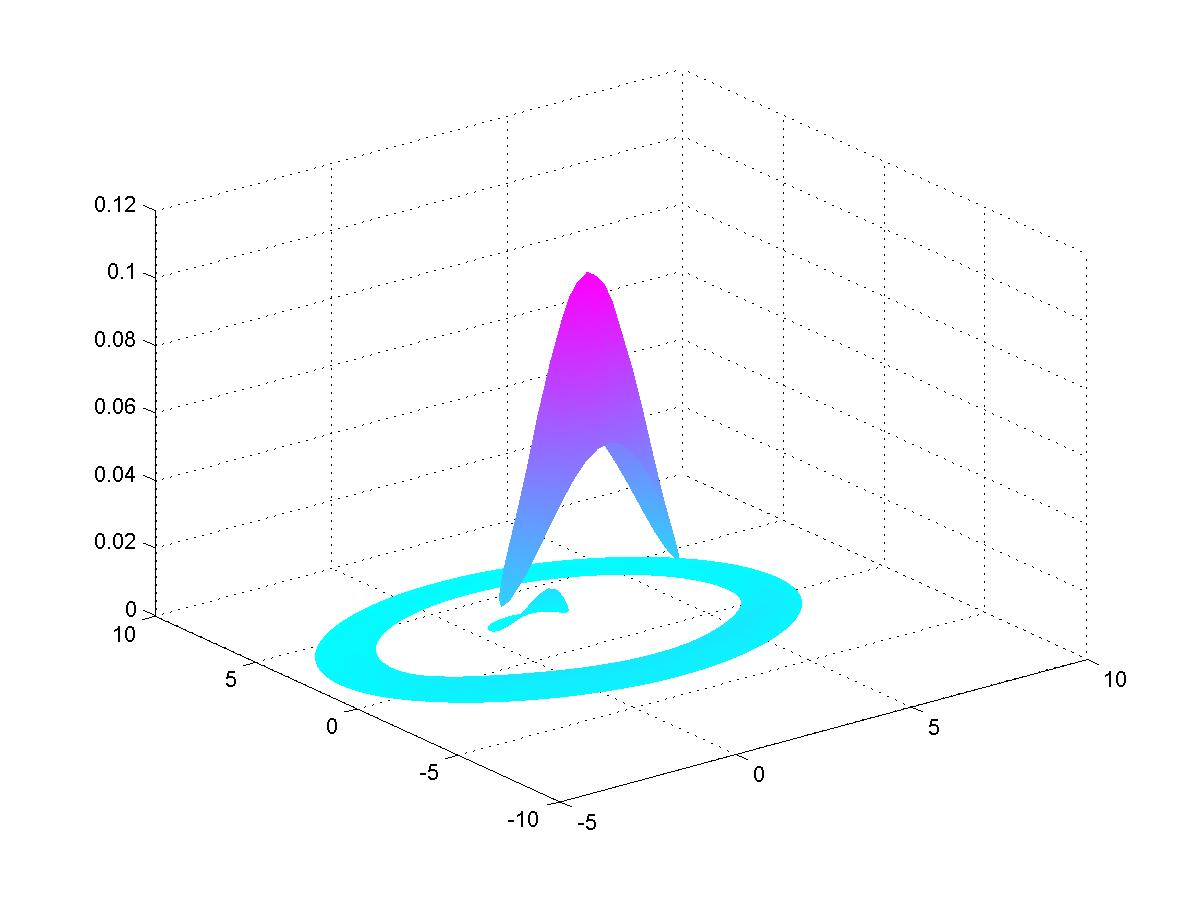
\includegraphics[width=0.28\linewidth]{eigspecdonut4} 
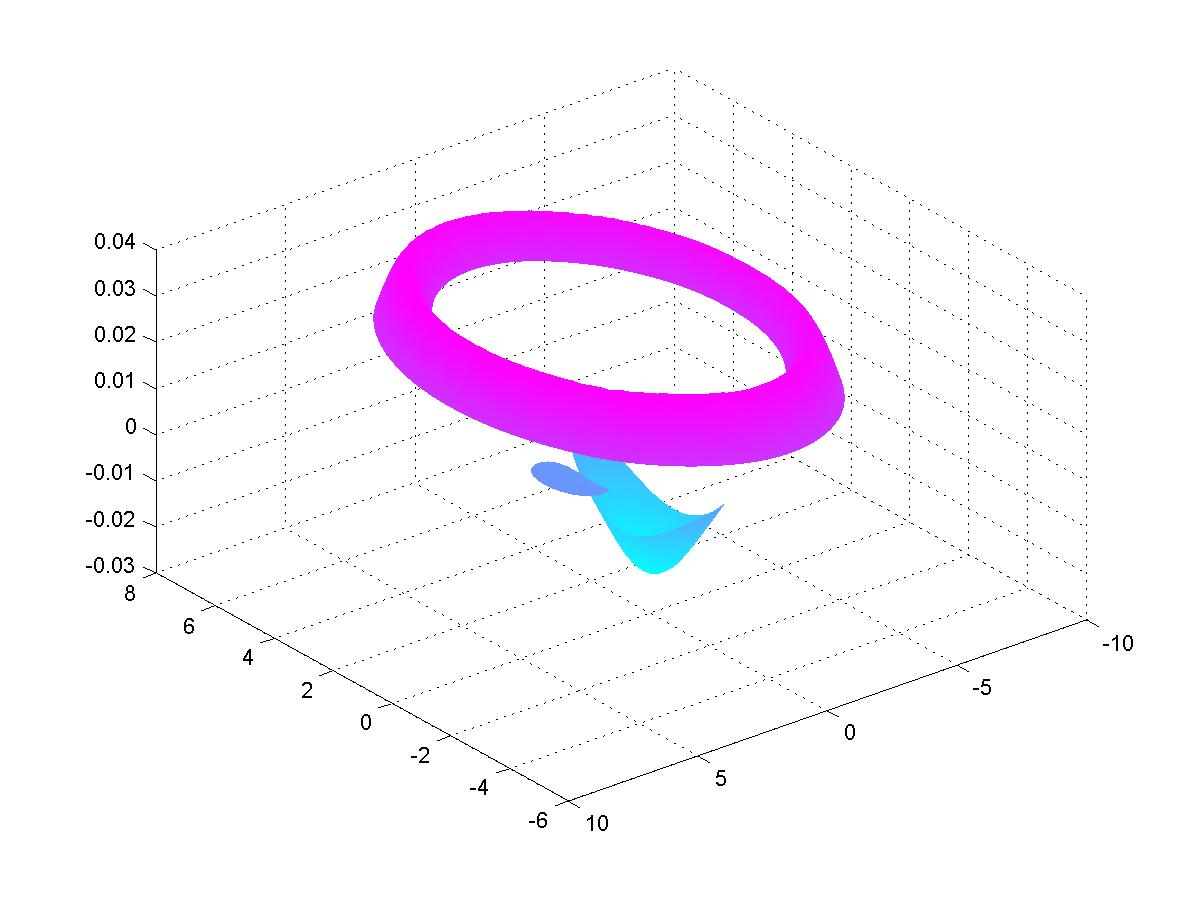
\includegraphics[width=0.28\linewidth]{eigspec2donut4} 
\end{center}

%%%%%%%%%%%%%%%%%%%%%%%%%%%
\vspace{-0.2cm}
We can prove that\footnote{Mouysset, S. and Noailles, J. and Ruiz, D., On an
interpretation of Spectral Clustering via Heat equation and Finite Elements
theory, Proceedings of International Conference on Data Mining and Knowledge
Engineering, 2010}:
\begin{enumerate}
\item eigenfunctions for bounded and free space Heat equation are asymptotically close when $t$ goes to 0,
\item difference between eigenvectors of $A$ and discretized eigenfunctions of
$K_t$ is %in $\mathcal{O}$ 
of an order of the distance between points inside the same cluster.
\end{enumerate}
}
\frame{\frametitle{Interpretation of Gaussian affinity matrix as
discretization of Heat kernel: towards the parallelization}

\begin{block}{Spectral Clustering as a "connected components" method}
%Eigenvectors of $A$ are an asymptotical discrete representation of $L^2$ eigenfunctions with support included in only one connected component.\\
\begin{itemize}
  \item Possibility to split the domain into subdomains;\\
  \item Applying Spectral Clustering into subdomains resumes in restricting
        the support of $L^2$ particular eigenfunctions;\\
  \item No alteration of the global partition: the eigenvectors carry the
        geometrical property, and so the clustering property.
\end{itemize}
\end{block}
}
%%%%%%%%%%%%%%%%%%%%%%%%%%%%%%%%%%%%
\frame{\frametitle{Domain decomposition strategy}
\begin{block}{}
\begin{itemize}
\item[$\rightarrow$]{\bf Parallel strategy: decomposition with overlaps}
\end{itemize}
\end{block}
\bigskip
\begin{multicols}{2}
\begin{figure}[htpb]
\begin{center}
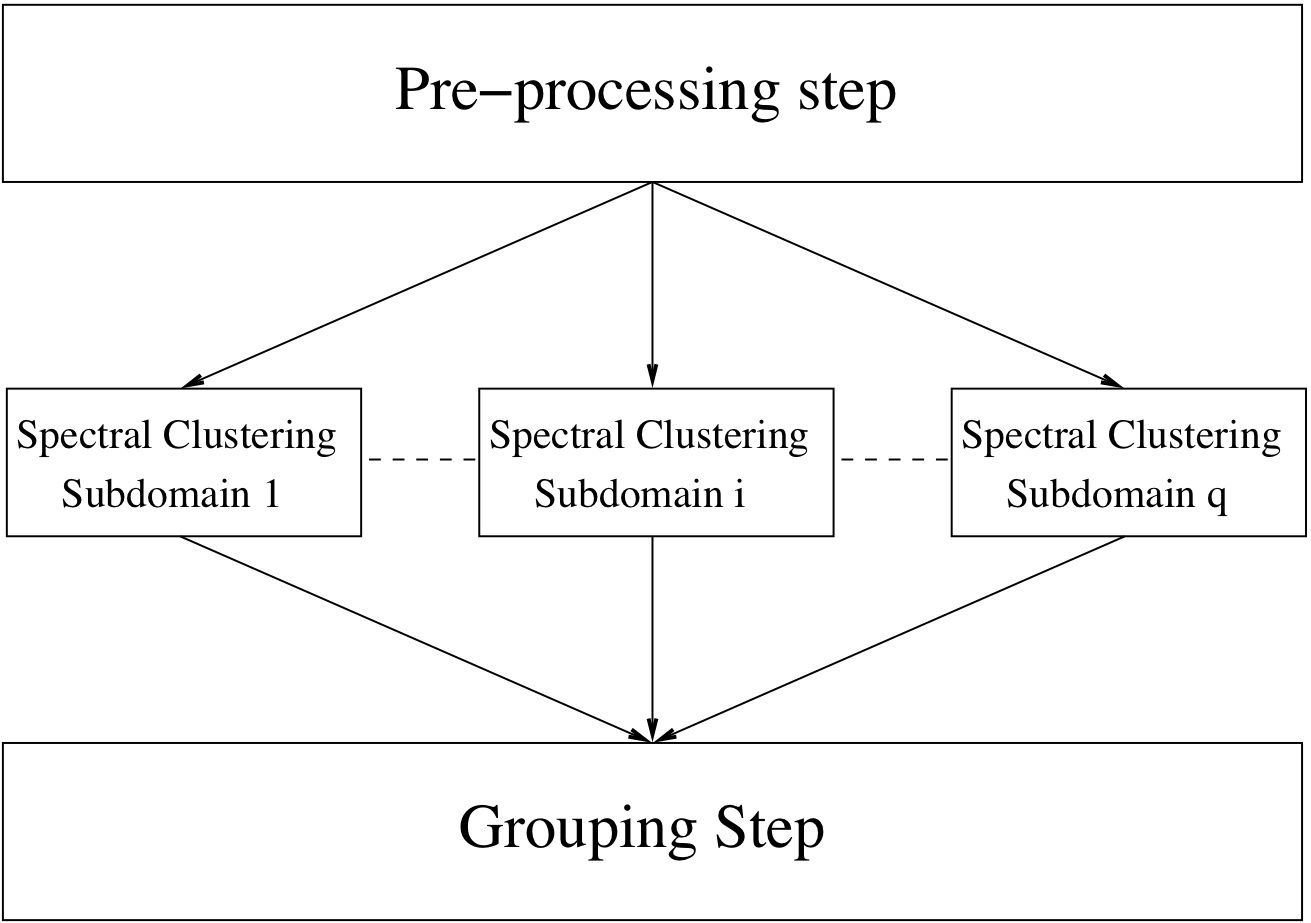
\includegraphics[width=0.8\linewidth]{intersectionq}
\caption{Principle of parallel Spectral clustering for $q$ subdomains} 
\end{center}
\end{figure}
\begin{figure}[!h]
\begin{center}
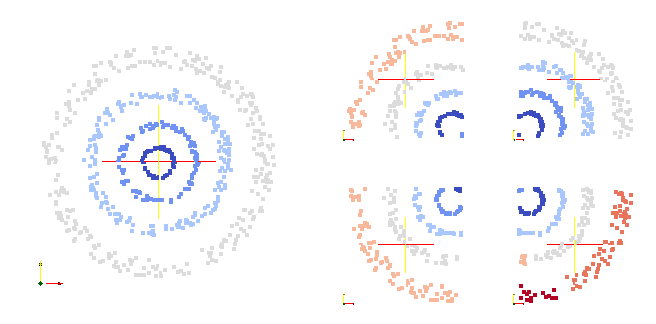
\includegraphics[width=1\linewidth]{cible_recouvrement2}
\caption{Target example: intersection and subdomains} 
\end{center}
\end{figure}
\end{multicols}

\begin{itemize}
 \item Total number of processes = q
 \item Grouping step: gather local partitions in a global partition
 (transitive relation\footnote{Mouysset, S. and Noailles, J., Ruiz, D. and Guivarch, R. On a strategy for Spectral Clustering with parallel computation,
\emph{VECPAR'10, High Performance Computing for Computational Science: 9th
International Conference}, 2010.})
\end{itemize}
}
%%%%%%%%%%%%%%%%%%%%%%%%%%%%%%
\frame{\frametitle{Sparsification of Spectral Clustering}


Despite the domain decomposition, the main computation cost problems are:\\
\begin{itemize}
\item Construction of the full affinity matrix by subdomain (memory cost):\\
\alert{$\qquad \rightarrow$ Sparsification of the affinity matrix by thresholding}
\item Computation of their largest eigenvectors (time cost): \\
\alert{$\qquad \rightarrow$ Adapted eigensolver for sparse matrix by using ARPACK }
\end{itemize}

\pause
\begin{block}{Thresholding interpretation }
Strengthens the piece-wise constancy of the dominant eigenvectors and so, the affinity between points among the same cluster and the separability between clusters
\end{block}
\begin{figure}[!h]
\begin{center}
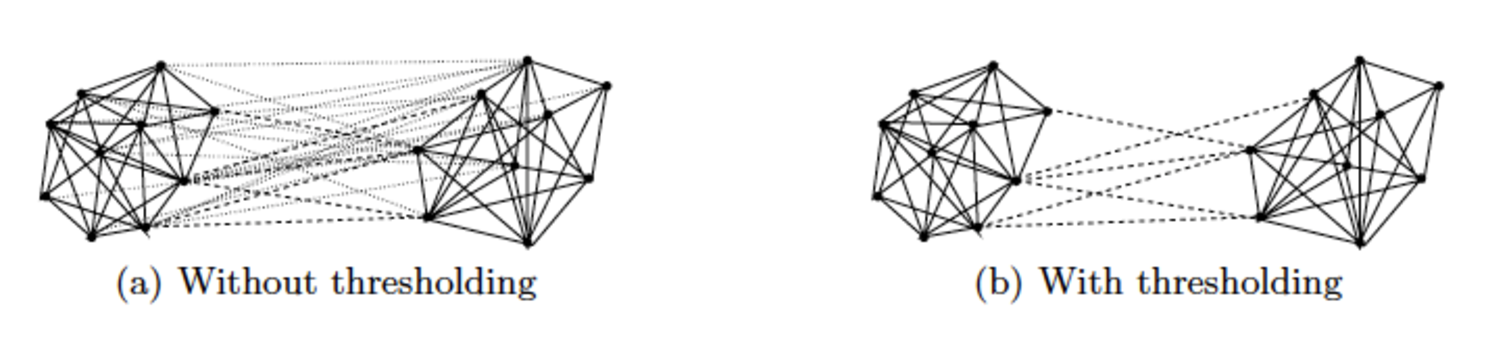
\includegraphics[width=1\linewidth]{InterpGraphes}
%\caption{Thresholding of  the weighted adjacency graph.} 
\end{center}
\end{figure}
\pause
\begin{itemize}
  \item we drop $A(i,j), i \neq j$ if $\left\|x_i-x_j\right\| <= threshold$.
\end{itemize}
}
%%%%%%%%%%%%%%%%%%%%%
\frame{\frametitle{Sparsification of Spectral Clustering: \textsc{Matlab} results}
\only<1>{
\begin{figure}[!h]
\begin{center}
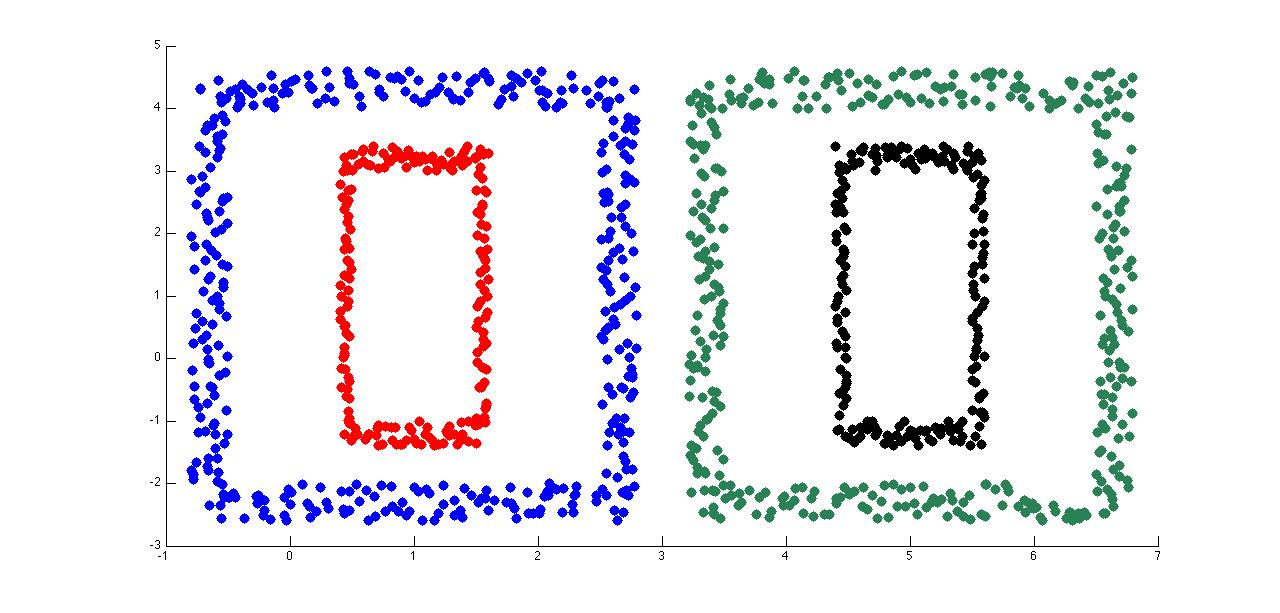
\includegraphics[width=0.6\linewidth]{4rectAffcoul}
\hspace{0.3cm}
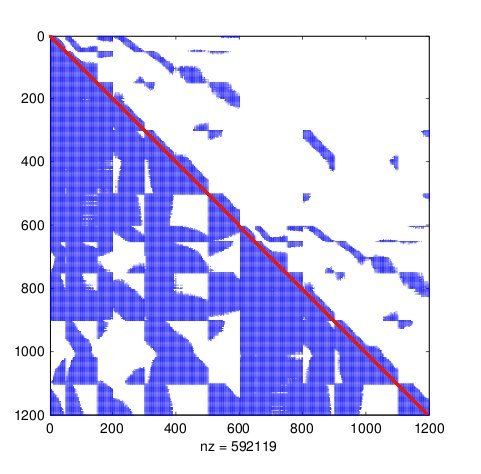
\includegraphics[width=0.35\linewidth]{4rectAffSpars}
\caption{Geometrical example: affinity matrix with and without thresholding} 
\end{center}
\end{figure}
\begin{itemize}
  \item $threshold = 10*\sigma$
\end{itemize}
}

\only<2>{
\begin{figure}[!h]
\begin{center}
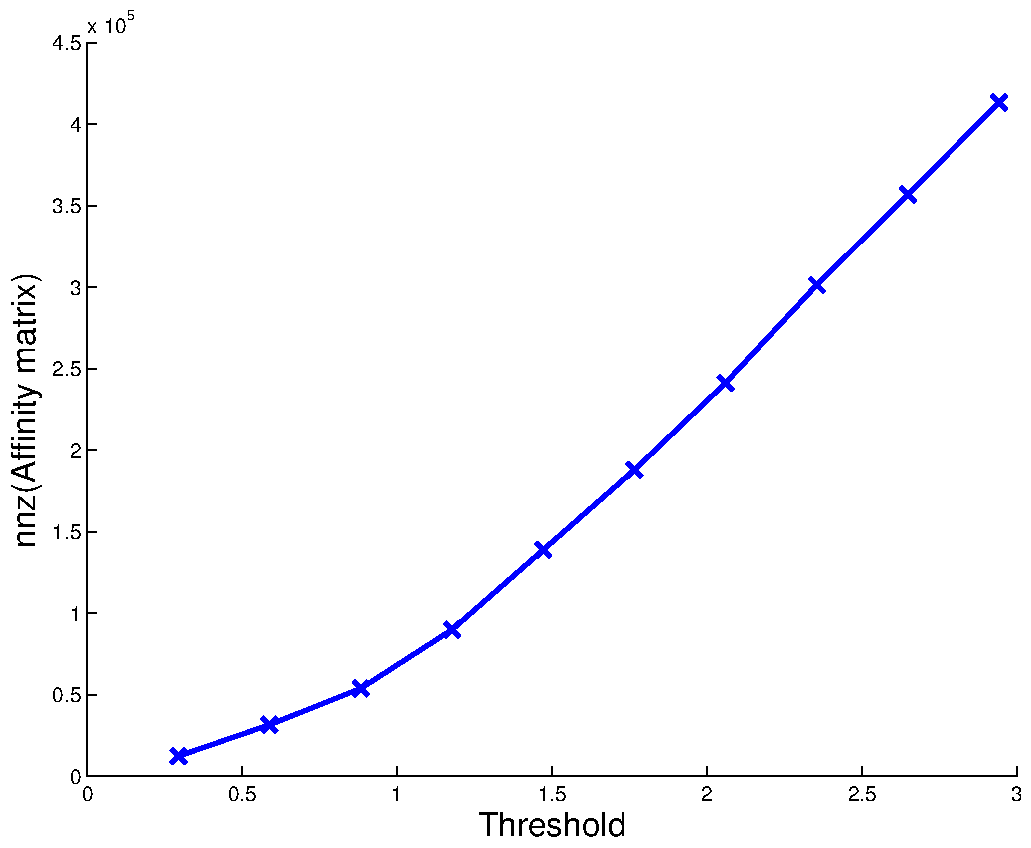
\includegraphics[width=0.4\linewidth]{Memo4rect}
\hspace{1cm}
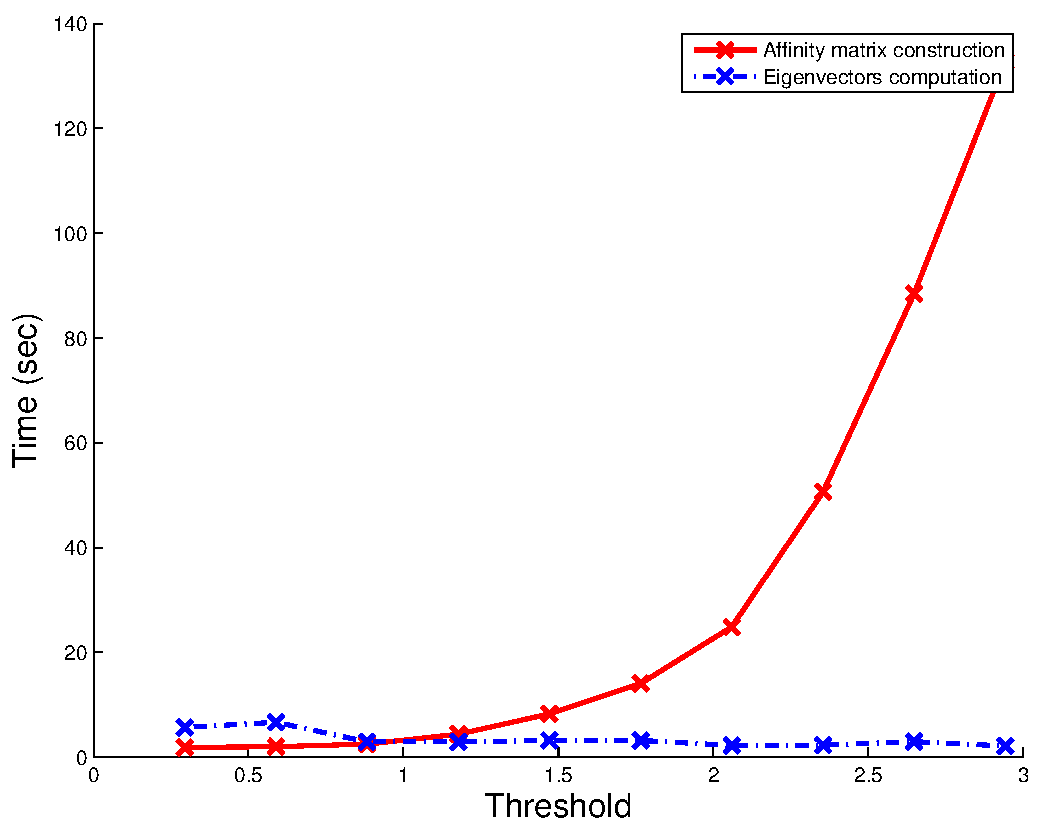
\includegraphics[width=0.4\linewidth]{Timings4rect}
\caption{Geometrical example: Memory cost and Timings function of the threshold} 
\end{center}
\end{figure}
construction of affinity matrix:
\begin{itemize}
  \item $A(i,j) = \displaystyle e^{-\left\|x_i-x_j\right\|^2/2 \bf \sigma^2}$
  \item we drop $A(i,j)$, if $\left\|x_i-x_j\right\| <= threshold$
  \item less computation (exponential)
\end{itemize}
}

}
%%%%%%%%%%%%%%%%%%%%%
%%%%%%%%%%%%%%%%%%%%%
\frame{\frametitle{Sparsification of Spectral Clustering: \textsc{Matlab} results}

\only<1>{
\begin{figure}[!h]
\begin{center}
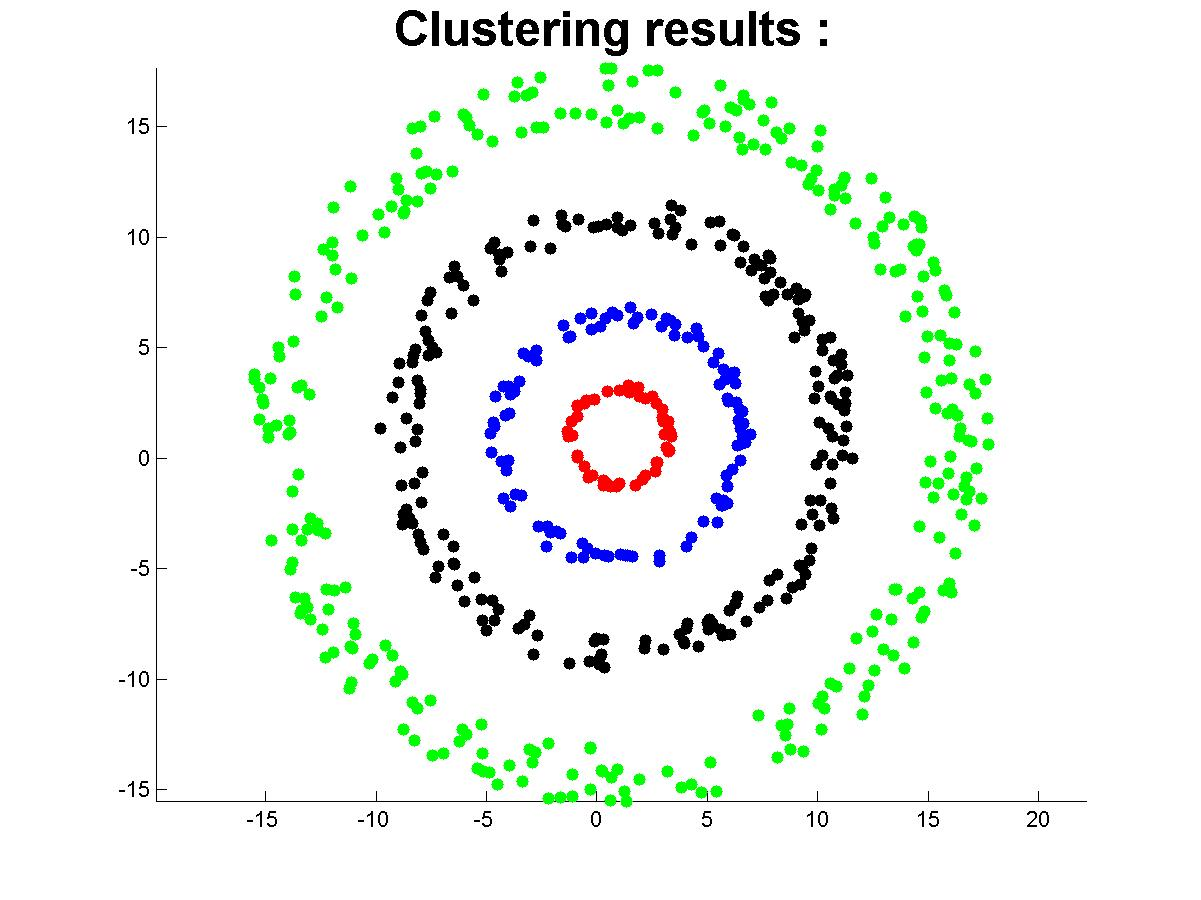
\includegraphics[width=0.45\linewidth]{cible}
\hspace{1cm}
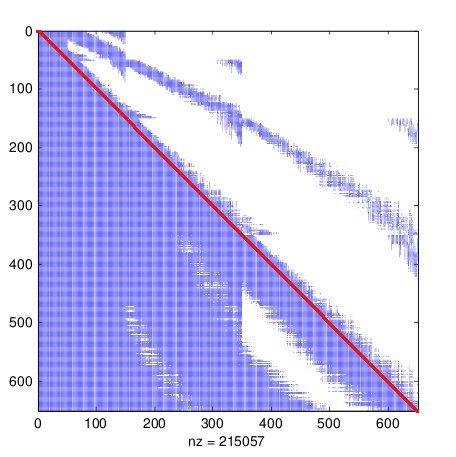
\includegraphics[width=0.35\linewidth]{CibleAffSpars}
\caption{Geometrical example: affinity matrix with and without thresholding} 
\end{center}
\end{figure}
\begin{itemize}
  \item $threshold = 10*\sigma$
\end{itemize}
}

\only<2>{
\begin{figure}[!h]
\begin{center}
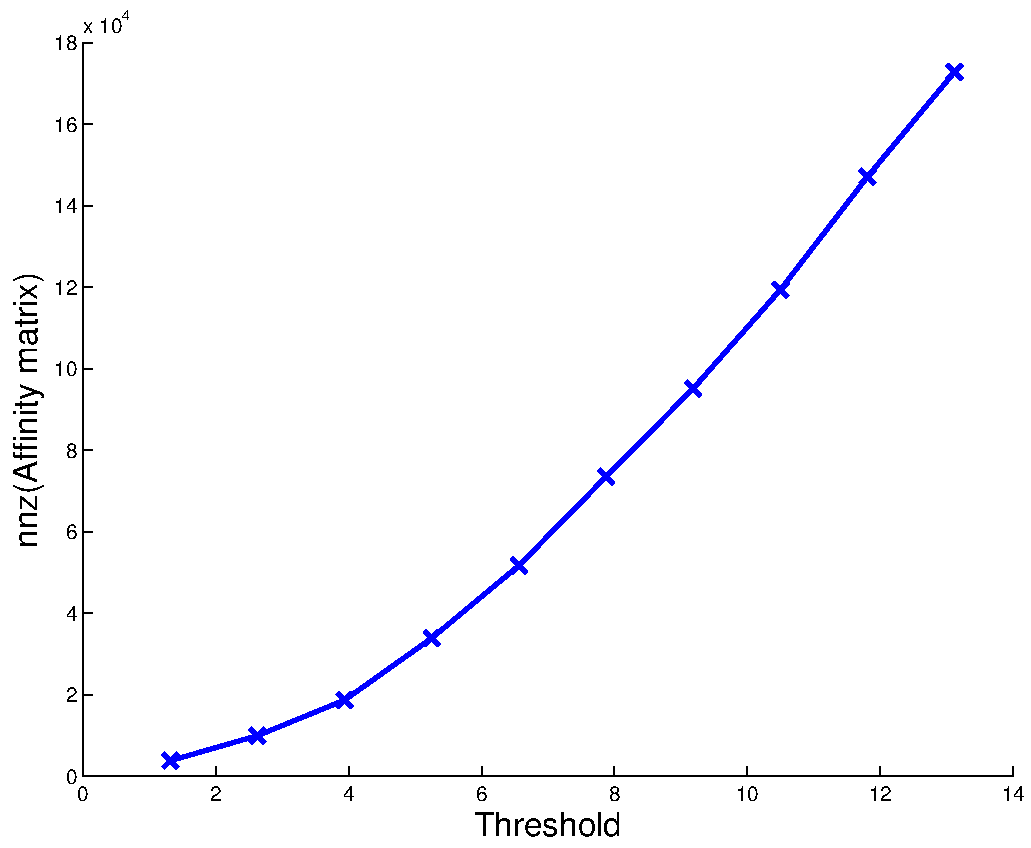
\includegraphics[width=0.4\linewidth]{MemoCible}
\hspace{1cm}
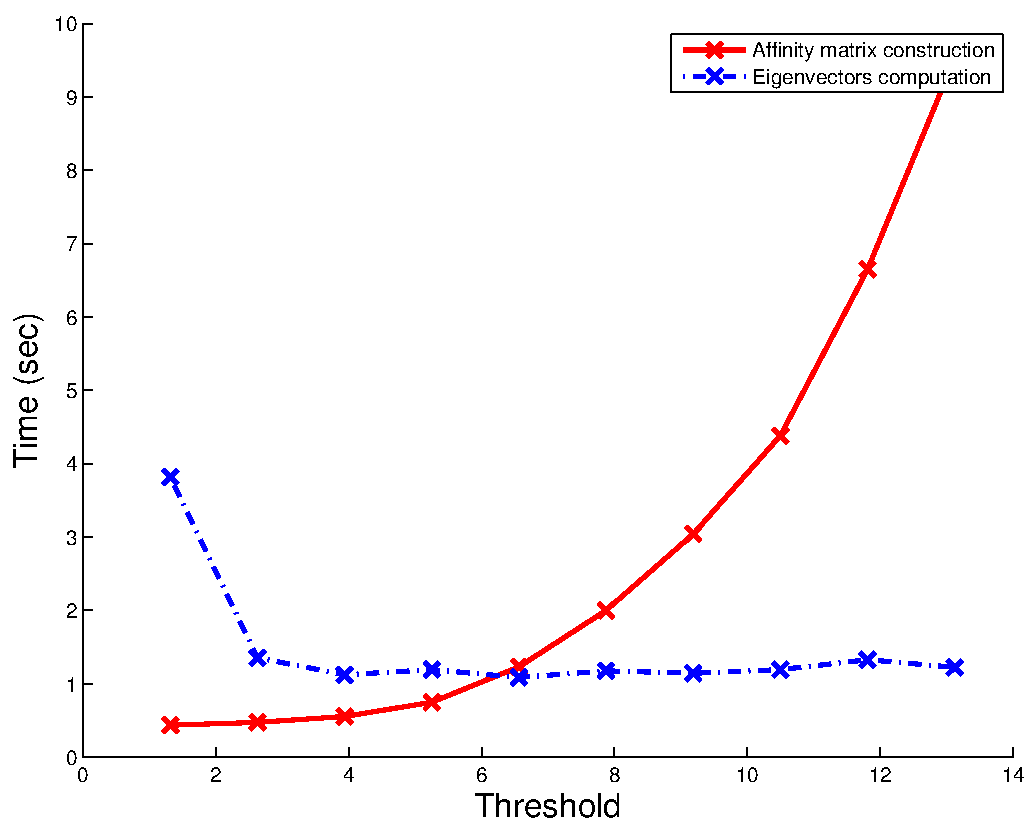
\includegraphics[width=0.4\linewidth]{TimingsCible}
\caption{Geometrical example: Memory cost and Timings function of the threshold} 
\end{center}
\end{figure}
}

}





%%%%%%%%%%%%%%%%%%%%%%
\frame{\frametitle{Application on images}

\begin{block}{Affinity measure}
The affinity measure between the pixel $(ij)$ and $(rs)$  includes both geometrical and color in affinity definition (3D or 5D data set):
\begin{equation}
d\left(I_{ij},I_{rs}\right)=\sqrt{\left(\frac{i-r}{l}\right)^2+\left(\frac{j-s}{m}\right)^2+\left(\frac{I_{ij}-I_{rs}}{256}\right)^2} \nonumber
\end{equation}

\end{block}
\begin{center}
\only<1>{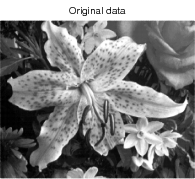
\includegraphics[width=4cm]{bouquet_lily_original}}
%\only<2>{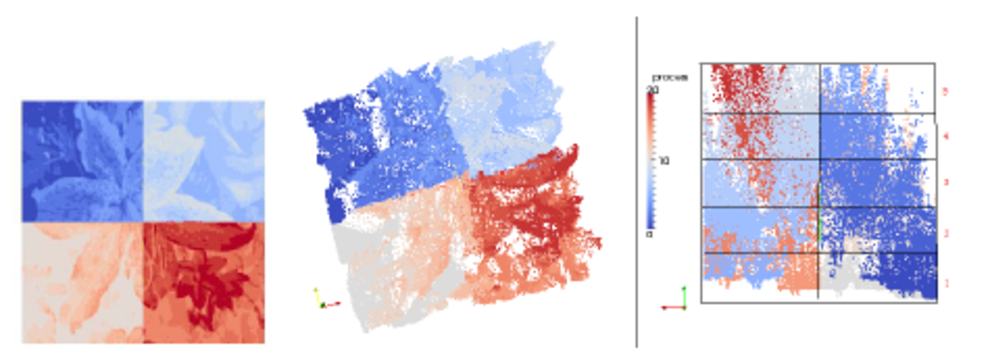
\includegraphics[width=1\linewidth]{decoupimage}}
\end{center}
}

%%%%%%%%%%%%%%%%%%%%%

\frame{\frametitle{Sparsification of Parallel Spectral Clustering: parallel
results\footnote{Hyperion cluster Altix ICE 8200 with 352 nodes (bi-Intel
"Nehalem" EX quad-core)}}

\begin{itemize}
  \item $ threshold = factor * \sigma$
  \item 20 subdomains
\end{itemize}

%Arthus 2

\begin{figure}[htpb]
\begin{center}
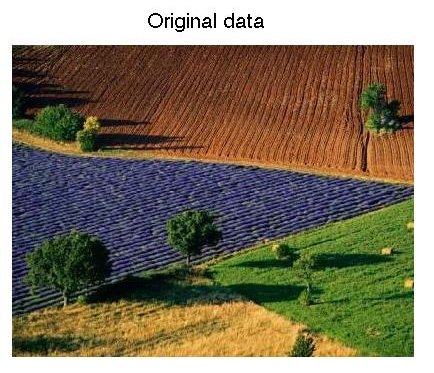
\includegraphics[width=0.3\linewidth]{Arthus2Data}
\hspace{0.3cm}
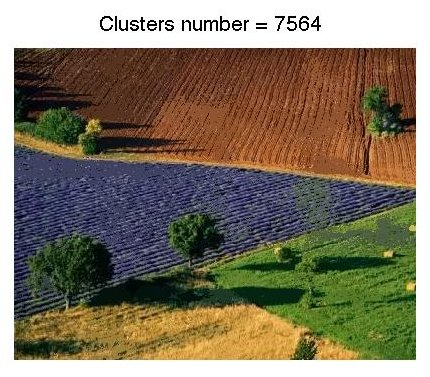
\includegraphics[width=0.3\linewidth]{Arthus2Full}
\hspace{0.3cm}
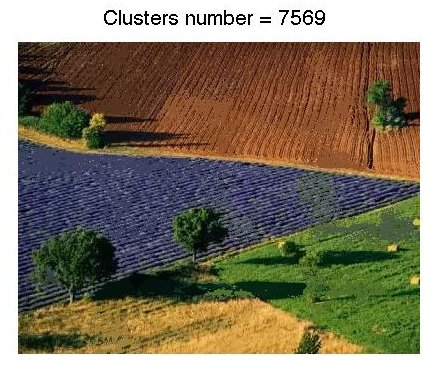
\includegraphics[width=0.3\linewidth]{Arthus2Sparse1}
\caption{Example of image segmentation: Original data, clustering result
without and with thresholding ($factor = 1$, $n=128612$ points)} 
\end{center}
\end{figure}

}

%%%%%%%%%%%%%%%%%%%%%%%%%%%%%%%%%%%%%%%%%%%%%�
\frame{\frametitle{Sparsification of Spectral Clustering: parallel results}

\begin{figure}[htpb]
\begin{center}
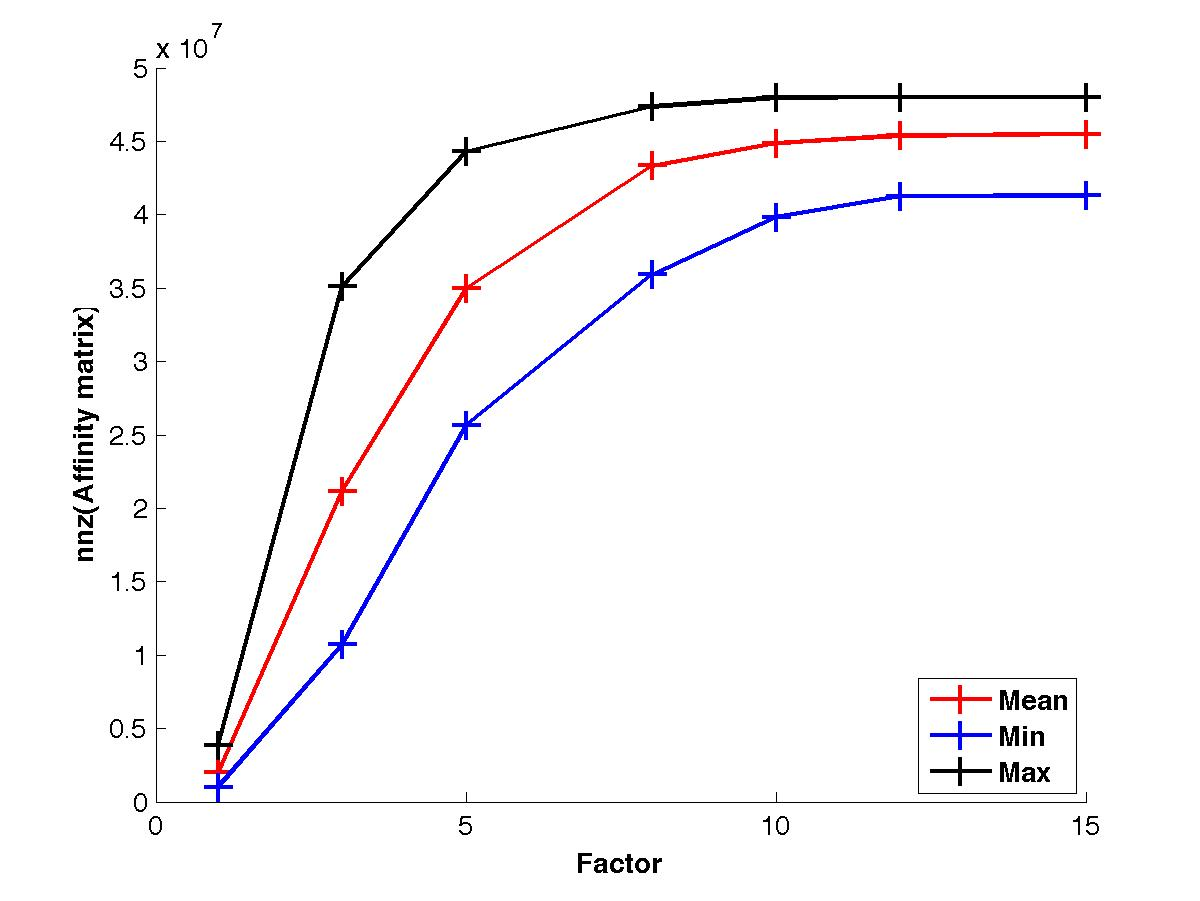
\includegraphics[width=0.8\linewidth]{Arthus2Stat}
\caption{Example of image segmentation: Memory cost function of the factor} 
\end{center}
\end{figure}

%\begin{itemize}
  %\item $ threshold = factor * \sigma$
  %\item 20 subdomains
%\end{itemize}

}
%%%%%%%%%%%%%%%%%%%%%%%%%%%%%%%
\frame{\frametitle{Conclusion and perspectives}

\begin{concl}
\begin{itemize}
\item Sparsification of affinity matrix construction by thresholding and using
eigensolver ARPACK in the parallel version of the code;
\item First parallel numerical results.\\
\end{itemize}
\end{concl}
\smallskip

\begin{block}{Perspectives}
\begin{itemize}
  \item Tune ARPACK to optimize the time to construct the eigenvectors;
  \item Choose of the threshold (factor) function of the distance $\sigma$
        that optimizes memory and computational costs with a good segmentation
        result;
        \begin{figure}[htpb]
\begin{center}
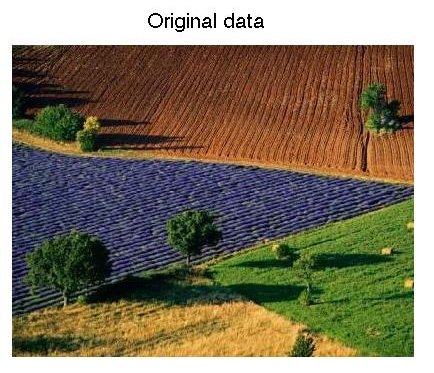
\includegraphics[width=0.3\linewidth]{Arthus2Data}
\hspace{0.3cm}
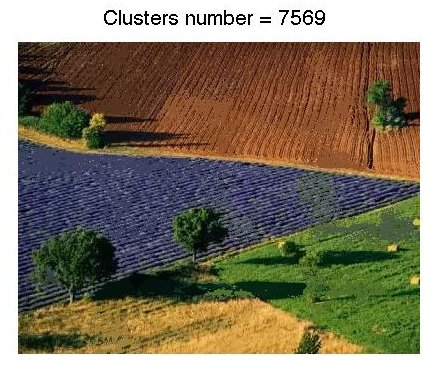
\includegraphics[width=0.3\linewidth]{Arthus2Sparse1}
\hspace{0.3cm}
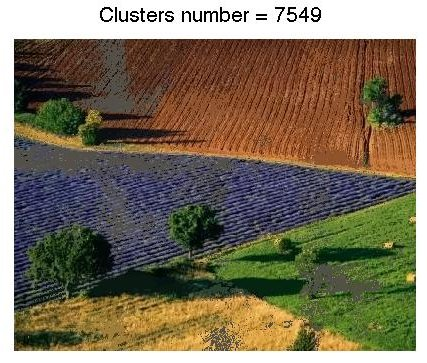
\includegraphics[width=0.3\linewidth]{Arthus2Sparse09}
\caption{Original data, clustering 
with thresholding ($factor = 1$ and $factor = 0.9$)} 
\end{center}
\end{figure}
\vspace{-0.3cm}
  \item Study of the robustness: bigger images, hyper-spectral images (more
  than 20M points)...
\end{itemize}
\end{block}
}

%%%%%%%%%%%%%%%%%%%%%%%%%%%%%%%%%
\frame{

\begin{center}
Thank you for your attention.
\end{center}
}

\end{document}
